%************************************************
\chapter{Learning to Accomplish Goals}\label{ch:learning_to_accomplish_goals}
%************************************************

\begin{quote}
  Problem-solvers must find relevant data.  How does the human mind
  retrieve what it needs from among so many millions of knowledge items?
  Different AI systems have attempted to use a variety of different
  methods for this.  Some assign keywords, attributes, or descriptors to
  each item and then locate data by feature-matching or by using more
  sophisticated associative data-base methods.  Others use
  graph-matching or analogical case-based adaptation.  Yet others try to
  find relevant information by threading their ways through systematic,
  usually hierarchical classifications of knowledge---sometimes called
  ``ontologies''.  But, to me, all such ideas seem deficient because it
  is not enough to classify items of information simply in terms of the
  features or structures of those items themselves.  This is because we
  rarely use a representation in an intentional vacuum, but we always
  have goals---and two objects may seem similar for one purpose but
  different for another purpose.
\end{quote}
\begin{flushright}
  --- \defcitealias{minsky:1991}{Marvin Minsky}\citetalias{minsky:1991}
\end{flushright}

% horvat: -^^^
%
%  very true
%  you could disuss it in paralell to the view that “mind
%  is a system always evolving” (Hoya, 2005)
%


The story of how I have gotten to this point along my current
trajectory of AI research is mostly idiosyncratic and not especially
interesting.  However, only in this story is there reason for my
current position.  As a young student, I grew up like most, learning
that the fundamental basis of my world is a real number domain of
space and time.  When I spread my arms I thought of real distances and
when I remembered the past and projected my future I thought of my
life as embedded in a real number line.  My first learning algorithms
were artificial neural networks, which because of their basis in real
numbers were close to my understanding of my physical self and the
physical world.  I used derivatives and integrals to predict events
within space and time.  I followed my intuitions from these numerical
instincts, which lead me to make probabilistic Gaussian mixture models
describing distributions of commonsense narratives over space and
time.  It was difficult to describe complete logics over these
relational numerical distribution spaces.  This model was an inference
model---nothing more.  My goal was to understand processes of
deliberation and reflective thinking over these narrative spaces, and
this inference model was going to be the basis of my next project.
What does a process look like in this narrative space?  I would need a
more complete logic in order to specify transition functions, in order
to simulate more general processes that could be deliberative.  I saw
my inference system, although complicated, as a reactive system
without much actual thought going on.  At this point, I read through
many of Marvin Minsky's old papers and discussed my project with him.
He was very skeptical that I would make much progress at all if I had
probabilistic representations as the fundamental representation in my
model.  Then, my goal was clearly before me.  At this point, I reread
almost all of Minsky's papers and his student's PhDs, including Gerry
Sussman's work on HACKER, a system that reflectively debugs its own
planning system.  I came to an epiphany at this point.  I saw Minsky's
Society of Mind and Emotion Machine as a detailed diagram for an
intricate new human programming language.  Every single part of the
history of AI suddenly fell into place given this overarching goal.
The representation for a process that I had been so confused about
with my work on probabilistic models suddenly slapped me in the face.
I had been staring at it for over twenty years.  The representation
for a process is the programming language itself.  As I approached
this new realization cautiously, I became more comfortable in my
conclusion through conversations with my close friend and theoretical
physicist, Julian Avila.  Through these discussions, I realized that
although much of physical science had turned to a fundamental
understanding of the world as probabilistic, I didn't agree.  A
probabilistic model must be based on something discrete that is
counted, in order to be rational.  Now, my task was clear, if I was
going to build something like a probabilistic model that counted, I
would first need something to count.  I abandoned my previous work
that treated probability as fundamental and worked on understanding
and trying to build Minsky's model, which I saw as a new programming
language that ``closes the loop'' not only once but twice---once for
perceiving and acting, and again for reflectively perceiving and
debugging the program itself.  In this PhD, I describe the resulting
learning system that does just this: closes the loop twice.

\section{Chapter Overview}

In this introductory chapter I will give an overview of the problem of
reflectively learning to accomplish goals.  First, I will develop the
assumption that any process that I choose under given constraints can
be reflectively monitored and useful information, e.g. beginning and
ending times, will be temporarily stored.  In other words, I assume
that my system natively supports procedural reflection for all
processes.  Given this assumption, I show in this chapter that the
problem of building a system that learns to accomplish goals in its
environment becomes a simple loop-less causal structure involving at
least four different types of learning.  These four types of learning
complete a circle of causal learning from goals through actions to
physical states and back to goals, but because of time, causality is
still in an ordered lattice structure beginning with goals as the
causal roots for all other knowledge.

In later chapters I will introduce experiments I have performed in
different physical problem simulations.  The first is a simple
proof-of-concept demonstration of my reflective learning algorithm in
a blocks world problem domain.  Also, I show my reflective
architecture extended to a larger physical reasoning domain, including
multiple AIs learning to cook together in a kitchen environment.
In this larger problem space, AIs can communicate high-level
procedures specified in a simple programming language that is shared
by the AIs, and refers to both mental and physical actions of the
AIs.

\section{The AI-Environment Model}

\begin{figure}[bth]
  \center
  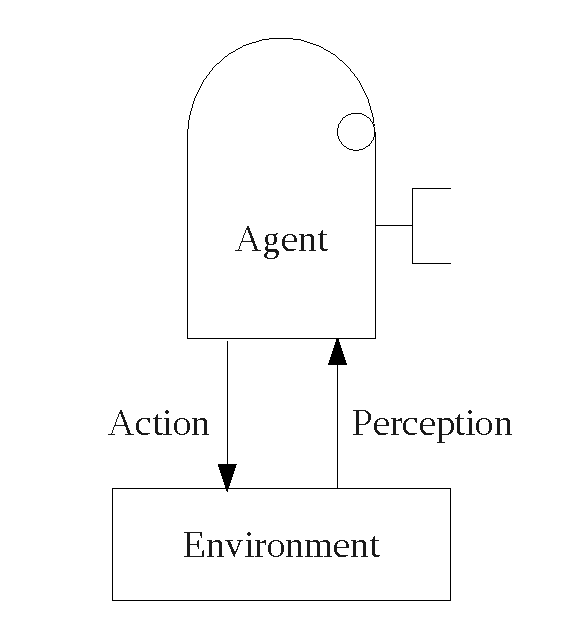
\includegraphics[height=5cm]{gfx/agent_environment}
  \caption[The AI-environment model]{The AI-environment model.}
  \label{fig:agent_environment}
\end{figure}

Figure~\ref{fig:agent_environment} shows the basic AI-environment
model.  In this model, I make a distinction between the environment
and the AI.  At any given time, the AI and the environment are
each represented as a specific static form of data.  Further, these
representations change over time, according to a given transfer
function.  I will treat this system as a deterministic system,
although one could imagine adding random variables to the transfer
function: the basic theory is the same.  It is easier to add
randomness to a deterministic theory than the opposite.  There are
also many benefits to developing a deterministic model with perhaps a
pseudorandom aspect because this allows for the repeatability of
scientific experiments, for which the model may be used as a metric.
The two processes communicate information along two channels: (1) an
action channel from the AI to the environment, and (2) a perception
channel from the environment to the AI.


\subsection{The State-Action Model}
\label{sec:state_action_model}

\begin{figure}[bth]
  \center
  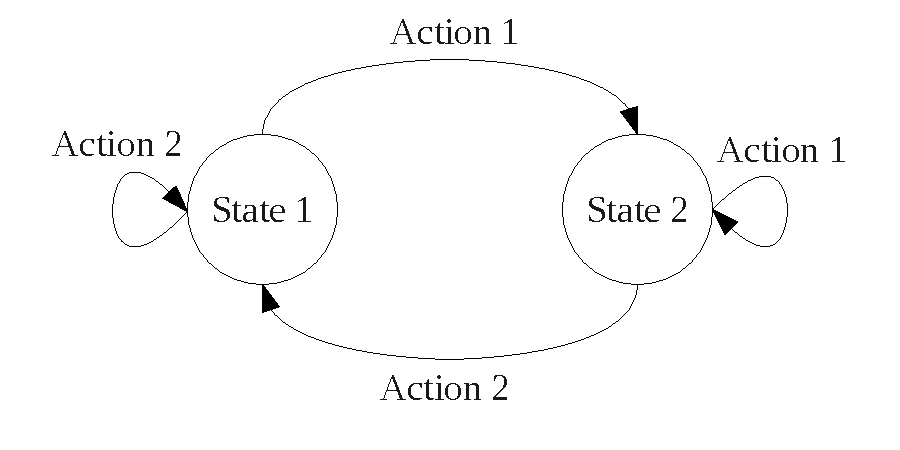
\includegraphics[width=6cm]{gfx/state_action}
  \caption[The state-action model]{The state action model.  Two states
    are represented by nodes and two actions are represented by edges
    from each of the two states.}
  \label{fig:state_action}
\end{figure}

The AI is in an environment, which is in a specific state.  My
AI performs an action, which can affect the state of the
environment.  Figure~\ref{fig:state_action} shows a simple \ac{FSM}
state-action model, which has two states for the environment and two
actions for the AI to perform in each of these states.  The
state-action model is a simple model for how actions map to changes in
the state of the environment.


\subsection{A Multiple AI-Environment Model}

\begin{figure}[bth]
  \center
  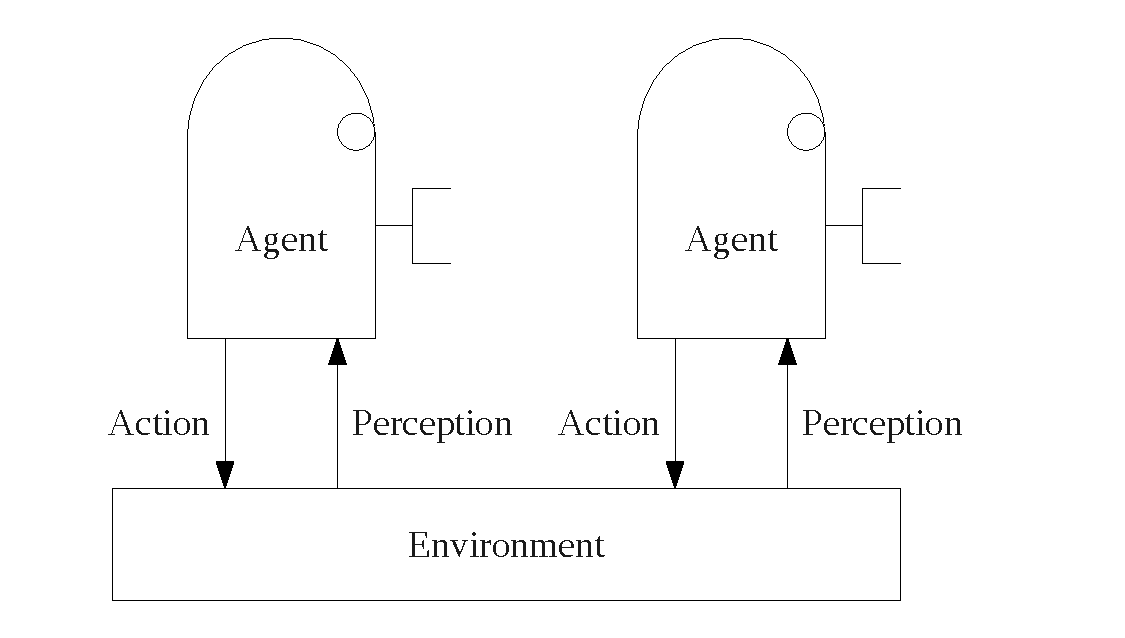
\includegraphics[height=5cm]{gfx/multiple_agent_environment}
  \caption[The multiple AI environment model]{The multiple AI environment model.}
  \label{fig:multiple_agent_environment}
\end{figure}

In order to model social intelligence, we introduce the multiple AI
environment model shown in
Figure~\ref{fig:multiple_agent_environment}.


\subsection{AI Process Communication}

Because AI processes can only directly act on and perceive the
environment, all communication between AI processes must occur
through the environment process.  We assume that AIs can
communicate some form of symbolic knowledge structure in the absence
of noise.  These representations are used to communicate processes
from one AI to another.  Specific examples of such a process
representation that we have used in our experiments are described in
more detail in
Sections~\ref{sec:serial_process_representation}--\ref{sec:parallel_process_representation}.


\subsection{A Relational State Representation}

\begin{figure}[bth]
  \center
  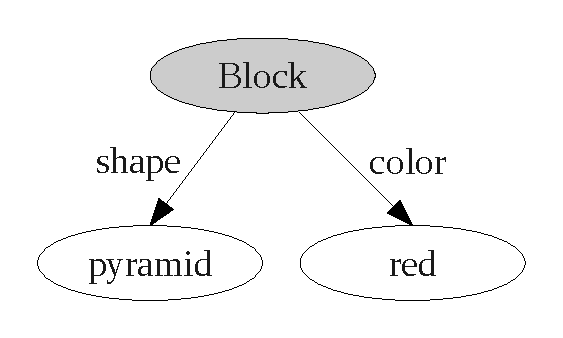
\includegraphics[height=3cm]{gfx/frame_representation}
  \caption[Frame-based relational representation]{Frame-based relational representation.}
  \label{fig:frame_representation}
\end{figure}

See Figure~\ref{fig:frame_representation}.

\subsection{Introducing Reflection Early in the Process}
\label{sec:introducing_reflection_early_in_the_process}

Now, I have introduced my problem as being divided into at least two
processes, at least one AI process and an environment process.
Further, I have introduced how a basic process may be thought of as an
\ac{FSM}.  At this point, I introduce a model for keeping track of the
changes in a computational process: reflective knowledge.  I
purposefully make this assumption before I define the details of the
AI model process because, in my approach, I would like to
reflectively reason about potentially any aspect of this AI
process.


\subsection{Reflective Knowledge}

\begin{figure}[bth]
  \center
  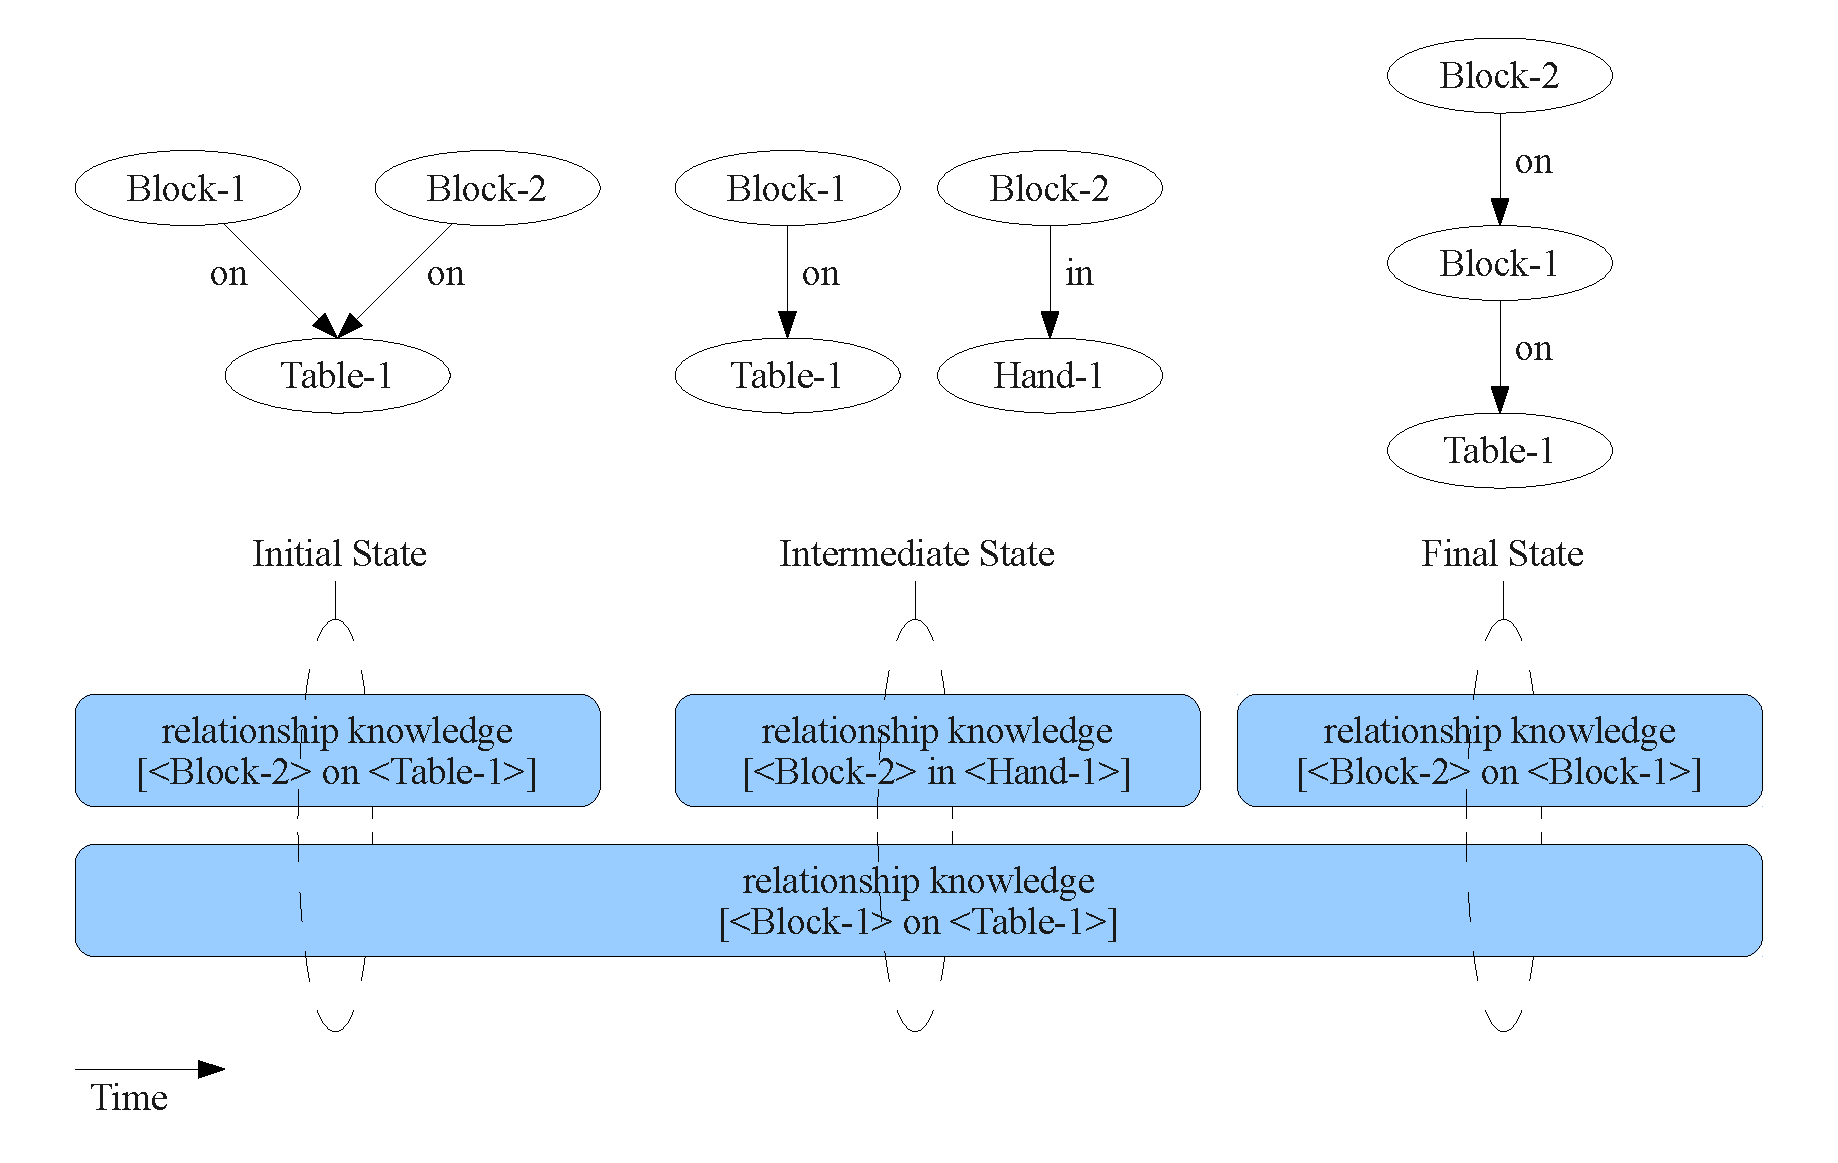
\includegraphics[width=12cm]{gfx/reflective_event_representation}
  \caption[A reflective event representation]{A reflective event representation shows the changes in a labeled graph.}
  \label{fig:reflective_event_representation}
\end{figure}


While the term meta-knowledge is used to describe the very general
idea of knowledge about knowledge, I use the term reflective knowledge
to refer to the specific type of meta-knowledge that refers to
knowledge about the changes to a knowledge structure.  If I keep track
of the changes to a knowledge structure, I can later integrate these
changes in order to obtain an equivalent form of that knowledge
structure as it was at any point in the past.\footnote{See
  Section~\ref{sec:what_is_a_computer} for a discussion of more
  realistic models of computation, including multiple-core and cluster
  models.}


\subsection{Frame Perceptions}

\begin{figure}[bth]
  \center
  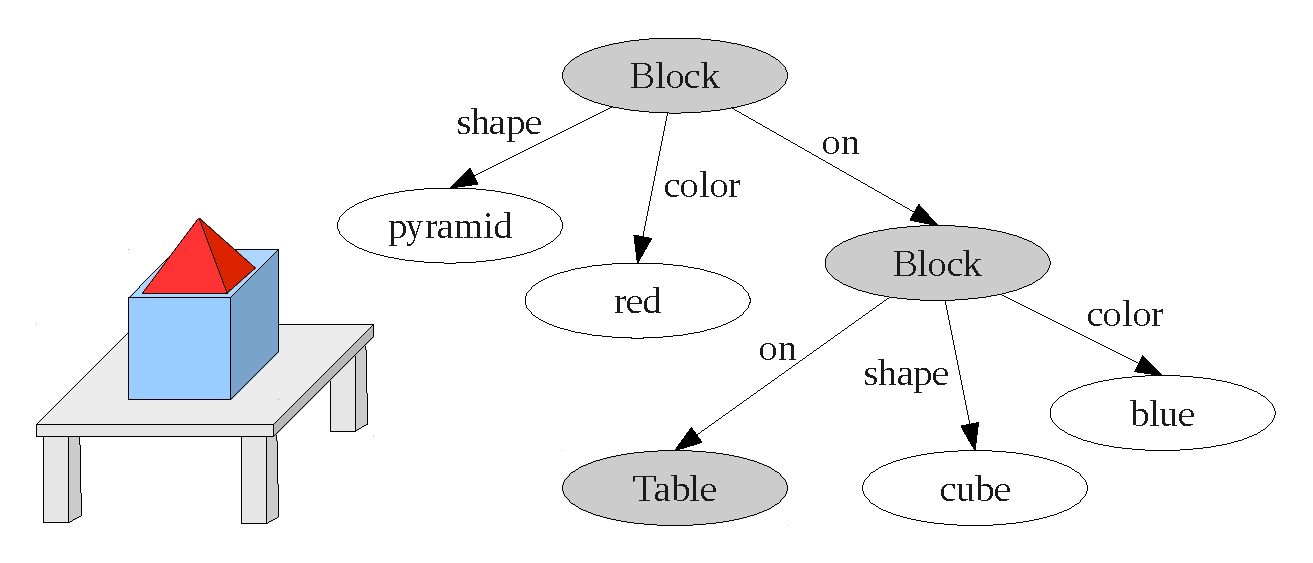
\includegraphics[height=5cm]{gfx/frame_perception}
  \caption[Collections of frames used as perceptual input to AI]{Collections of frames used as perceptual input to AI.}
  \label{fig:frame_perception}
\end{figure}

See Figure~\ref{fig:frame_perception}.


\subsection{Partially Observable State Model}

\begin{figure}[bth]
  \center
  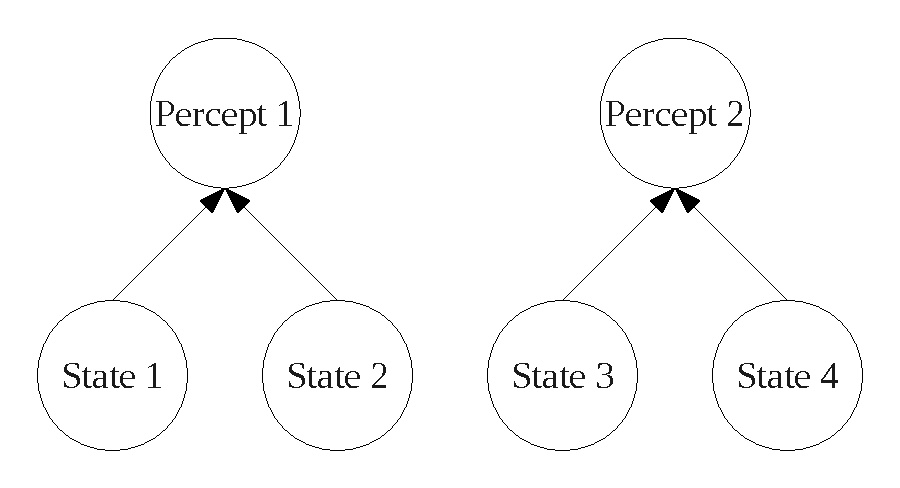
\includegraphics[width=6cm]{gfx/partially_observable}
  \caption[The partially observable state model]{The partially observable model.}
  \label{fig:partially_observable}
\end{figure}

\begin{figure}[bth]
  \center
  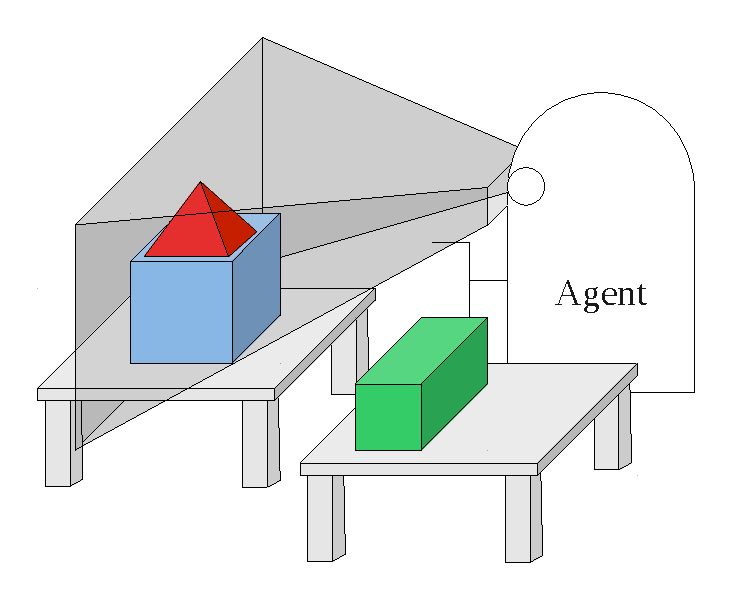
\includegraphics[height=5cm]{gfx/partial_frame_perception}
  \caption[The state of the environment is only partially
    observable]{The state of the environment is only partially
    observable.}
  \label{fig:partial_frame_perception}
\end{figure}

The AI process does not have complete access to the state of its
environment.  The AI's perceptual stream of information depends on
the state of the environment, but it is a function of the environment
and not the actual state of the environment.  In other words, the
perceptual state that is communicated from the environment to the
AI is an injective function mapping the environment to the
perception of the AI.  See
Figures~\ref{fig:partially_observable}~and~\ref{fig:partial_frame_perception}
for two examples of partially observable environments.


\subsection{AI Abstract Physical Model}

\begin{figure}[bth]
  \center
  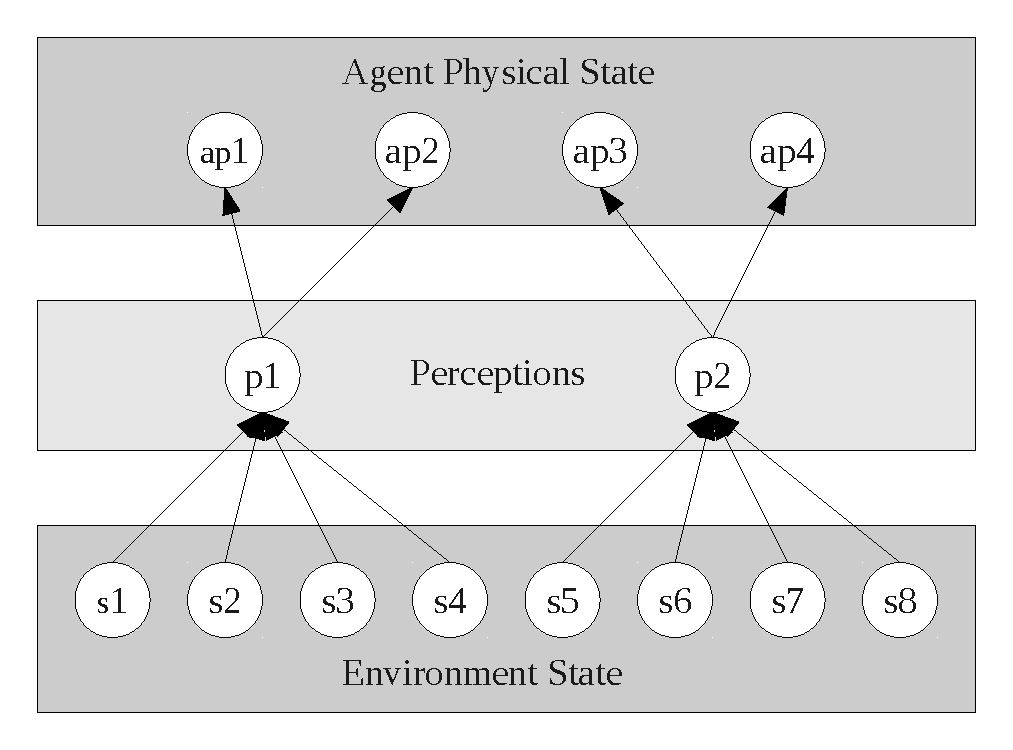
\includegraphics[width=8cm]{gfx/environment_perception_physical}
  \caption[The AI has an abstract physical model of the
    environment]{The AI has an abstract physical model of the
    environment.}
  \label{fig:environment_perception_physical}
\end{figure}

See Figure~\ref{fig:environment_perception_physical}.


\subsection{A Physical Goal Representation}

\begin{figure}[bth]
  \center
  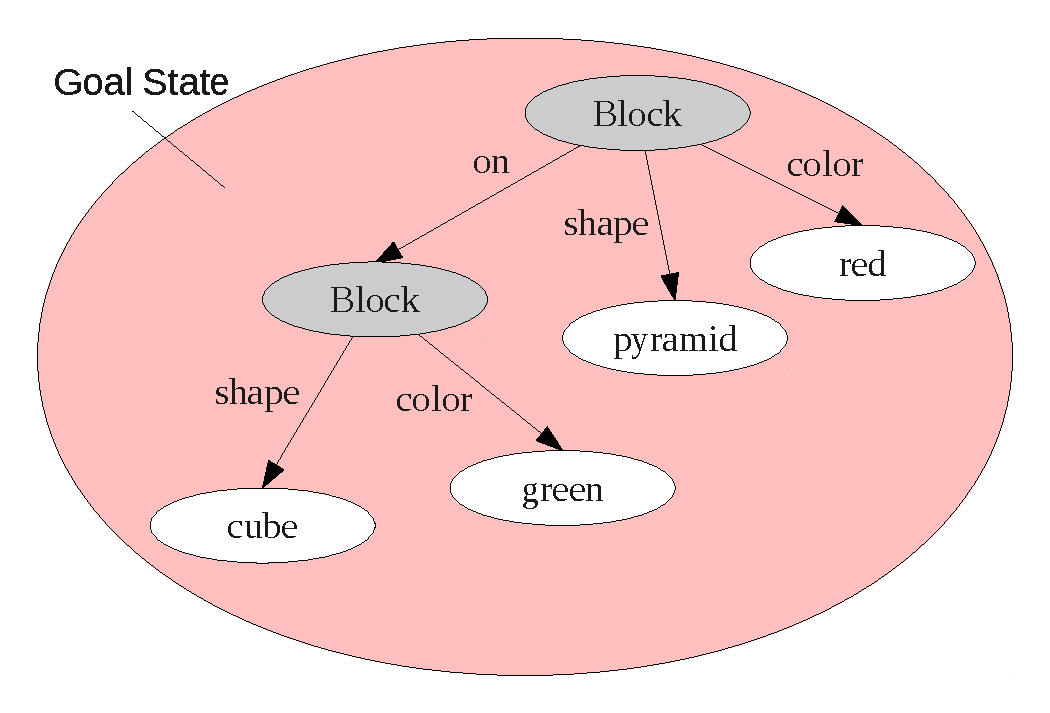
\includegraphics[height=4cm]{gfx/goal_state}
  \caption[A physical goal representation]{A physical goal
    representation is a structural relationship that may or may not
    currently exist within the physical knowledge base.}
  \label{fig:goal_state}
\end{figure}

See Figure~\ref{fig:goal_state}.


\section{The Reflective Learning Cycle}

I have now introduced the definitions for my relational state space,
along with how reflective tracing, given certain assumptions, allows
the creation of reflective event representations of the action
resources within the AI's mind.

In this section, I will describe how these representations and
reflective event representations can be used to reflectively learn the
different types of knowledge used for planning.

\begin{figure}[bth]
  \center
  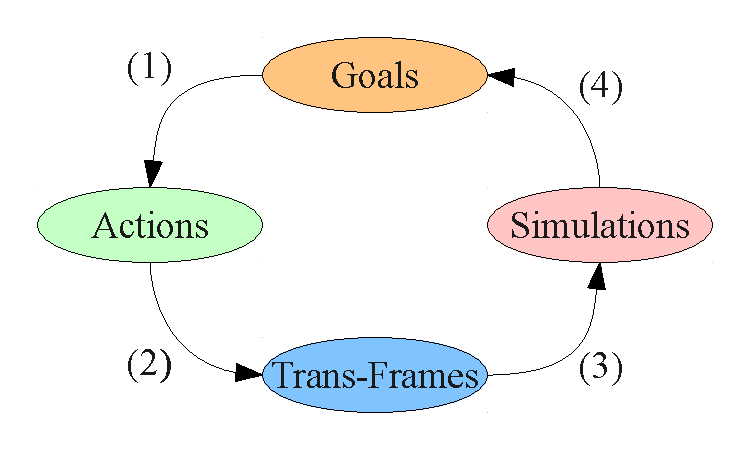
\includegraphics[width=6cm]{gfx/learning_to_plan-four_step_cycle}
  \caption[Learning to plan four step cycle]{Learning to plan four step cycle.}
  \label{fig:learning_to_plan-four_step_cycle}
\end{figure}

Figure~\ref{fig:learning_to_plan-four_step_cycle} shows the abstract
four-step learning to plan cycle.  Planning is an arbitrarily
complicated process, but with these four steps I have created basic
semantic divisions between the types of knowledge involved in
reflectively learning to plan.  These basic divisions in the learning
process can be summarized as:

\begin{enumerate}
\item{Changing goal knowledge initiates causal learning.}
\item{Physical precondition concept for goal occurrence is refined.}
\item{Physical transition concepts for simulating action resource are refined.}
\item{Physical concept for goal occurrence is refined.}
\end{enumerate}

\begin{figure}[bth]
  \center
  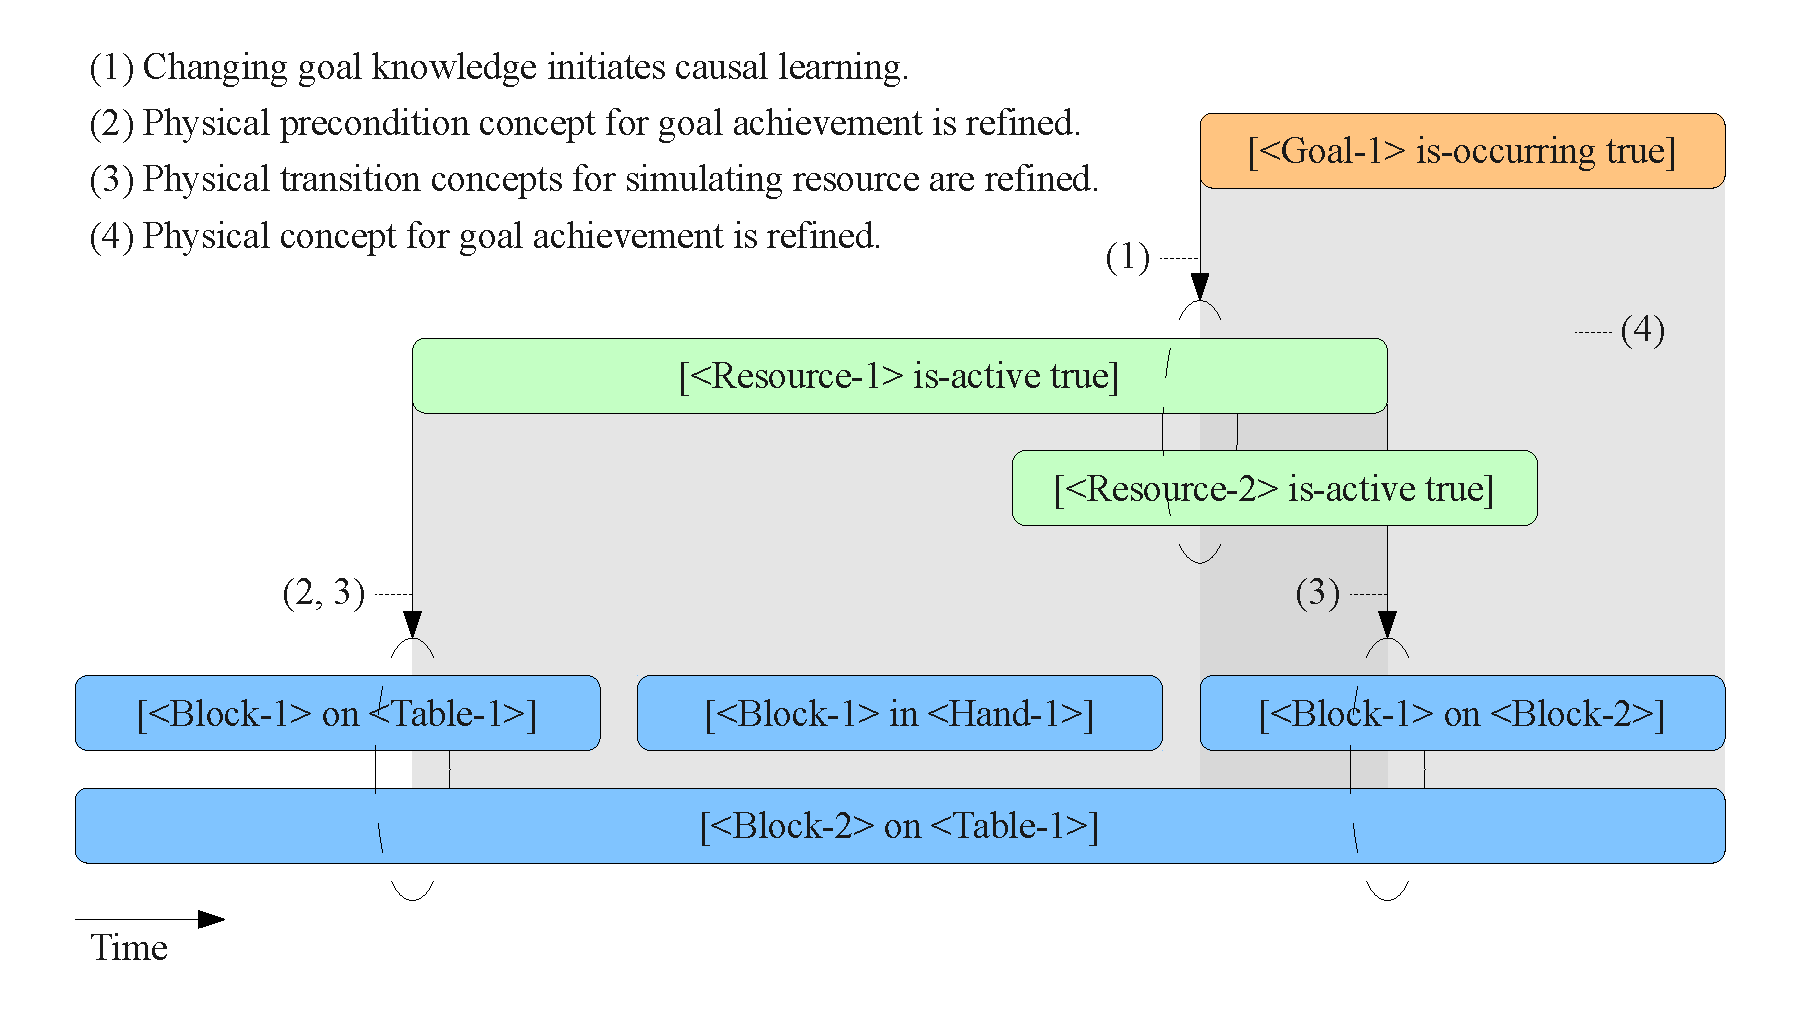
\includegraphics[width=12cm]{gfx/learning_to_plan}
  \caption[The reflective learning cycle]{The reflective learning
    cycle is a way to learn knowledge used to plan toward goals that
    maintains the causal dependency structure of the knowledge.}
  \label{fig:learning_to_plan}
\end{figure}

A system without a goal has no reason to learn the effects of its
actions.  Figure~\ref{fig:learning_to_plan} shows how this process of
learning causal models relating reflective states to physical states
is a fundamentally goal-driven process.  We show how this goal
prediction process leads to at least a four step causal chain of
knowledge learning.  It is important to point out that although the
learning process is a cycle over time, this ends up creating a causal
structure for knowledge dependency without loops---a critical property
in general to maintain for any causal representation.

These four goal-oriented cyclical learning steps build four of the
major types of knowledge that my goal-oriented inference and planning
system uses.  Let us now briefly introduce these four types of
knowledge before going into a more thorough explanation of the utility
of each.

\begin{enumerate}

\item{Goal-oriented action hypotheses: focuses and constrains the
  initial action learning search.}

\item{Action physical precondition goal occurrence hypotheses: allows
  predicting whether or not an action will accomplish the given goal
  under a given physical precondition.}

\item{Action physical precondition trans-frame hypotheses: allows for
  physically simulating the given action in a given physical state.}

\item{Physical hypotheses for predicting goal occurrence: allows for
  predicting if a given physical state implies that the goal is
  occurring.}

\end{enumerate}

Note that there are two different concepts of time that are displayed
in Figure~\ref{fig:learning_to_plan}.  It is important to not confuse
these.  The first kind of time is represented by the sequence of
change events in the knowledge structure that was reflectively traced
in order to generate the temporal event representation shown in the
figure.  This first time is represented and labelled as the horizontal
axis in the figure.  The second kind of time represented in the figure
is represented by the enumeration of the four learning steps.  This
learning process is a reflective learning process because it learns
from reflective knowledge gathered from tracing processes.

In the following four sections, we will describe the utility of each
of these four different types of learned knowledge in more detail.

\subsection{Causal Action Hypotheses}
\label{sec:goal_oriented_action_hypotheses}

\begin{figure}[bth]
  \center
  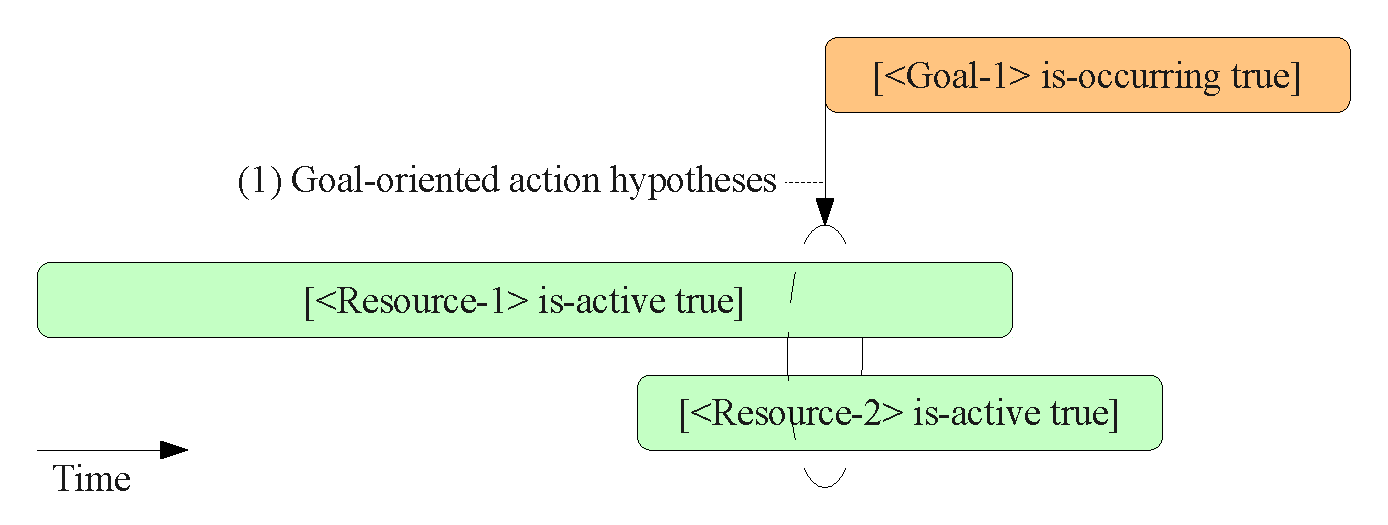
\includegraphics[width=11cm]{gfx/learning_to_plan-1-goal_oriented_action_hypotheses}
  \caption[Goal-oriented action hypothesis knowledge]{Goal-oriented action hypothesis knowledge.}
  \label{fig:goal_oriented_action_hypotheses}
\end{figure}

\marginpar{\emph{learning goal}: focusing learning on a subset of the state space.}

Figure~\ref{fig:goal_oriented_action_hypotheses} shows the first step
of the reflective learning cycle.  This first step of the learning
cycle is caused reflectively by the goal event beginning to exist.
When a goal event comes into existence, a reflective process
monitoring this goal knowledge makes a list of potential actions that
might be useful for causally predicting this goal condition in the
future.  In the figure we can see that a simple interval-point
intersection operation between the beginning point of the goal event
and any action event interval is enough to generate two actions as
initial causal hypotheses.  See
Section~\ref{sec:goal_oriented_action_hypotheses_generation_techniques}
for details on the techniques that I used for generating goal-oriented
action hypotheses in my system.


\subsection{Action Goal Occurrence Hypotheses}

\begin{figure}[bth]
  \center
  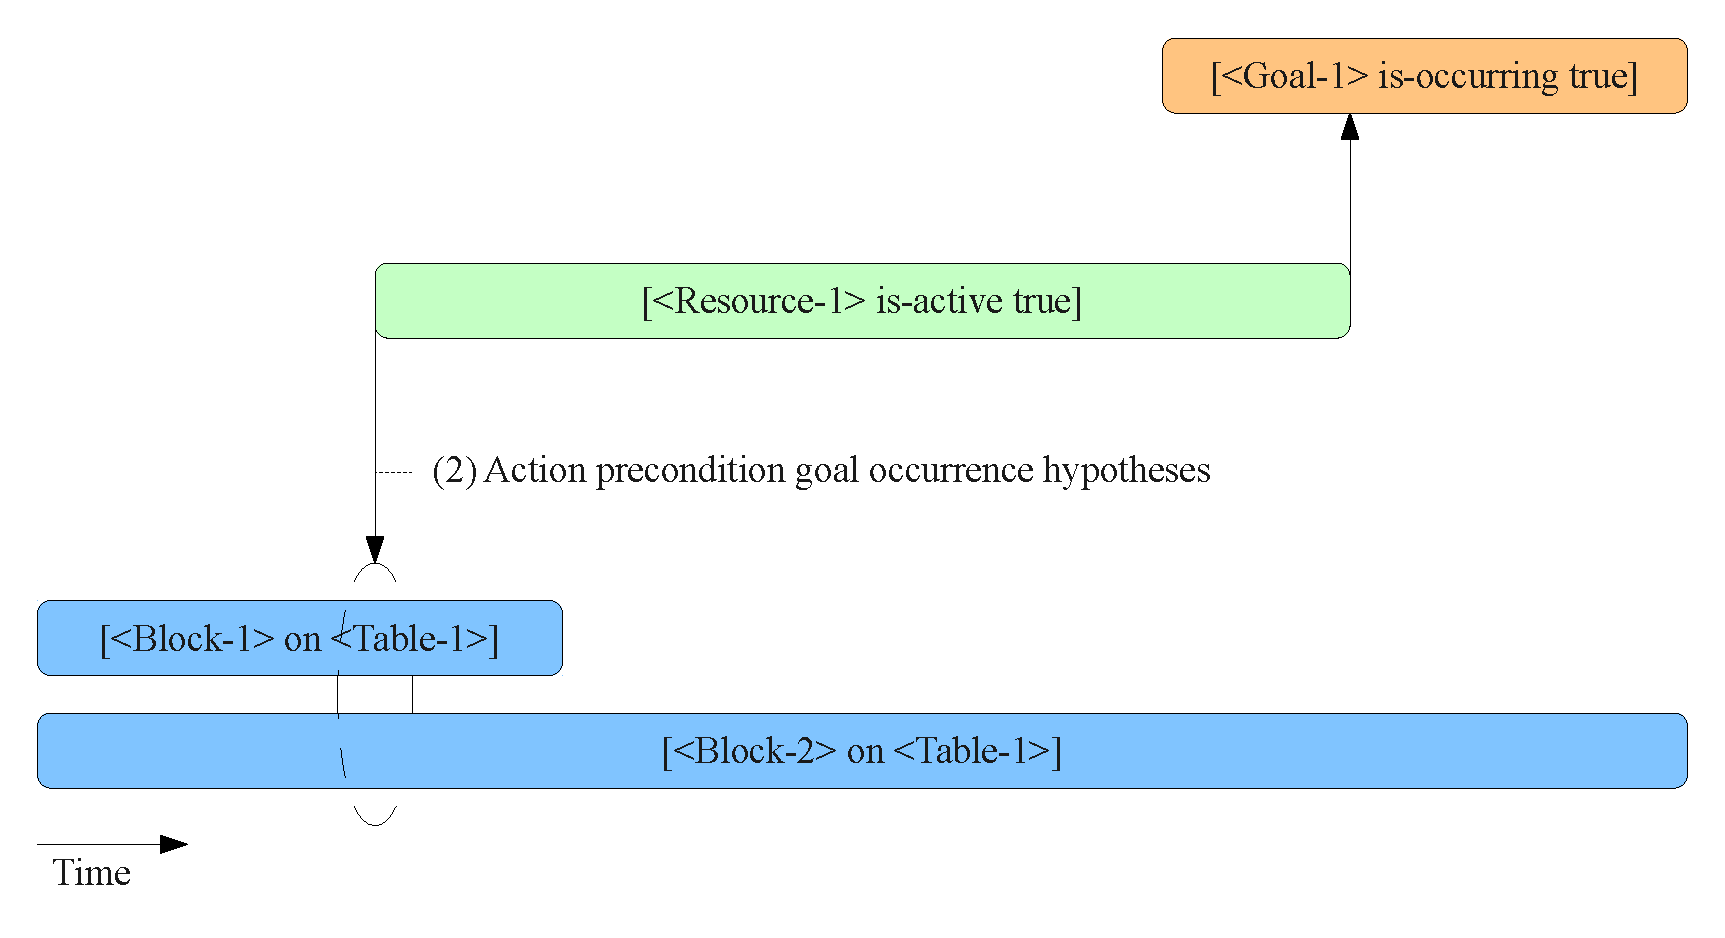
\includegraphics[width=11cm]{gfx/learning_to_plan-2-action_precondition_goal_occurrence_hypotheses}
  \caption[Action precondition goal occurrence hypotheses]{Action
    precondition goal occurrence hypotheses can be learned from these
    reflective representations.}
  \label{fig:action_precondition_goal_occurrence_hypotheses}
\end{figure}

Action precondition goal occurrence hypotheses are a form of knowledge
that is learned in order to predict whether or not a goal will be
occurring if a given action is taken in a given conceptual category of
a given abstraction of the state space.
Figure~\ref{fig:action_precondition_goal_occurrence_hypotheses} shows
the reflective event representations that can be used to learn this
type of knowledge.

\subsection{Action Trans-Frame Hypotheses}
\label{sec:learning_trans_frames_for_events}

\begin{figure}[bth]
  \center
  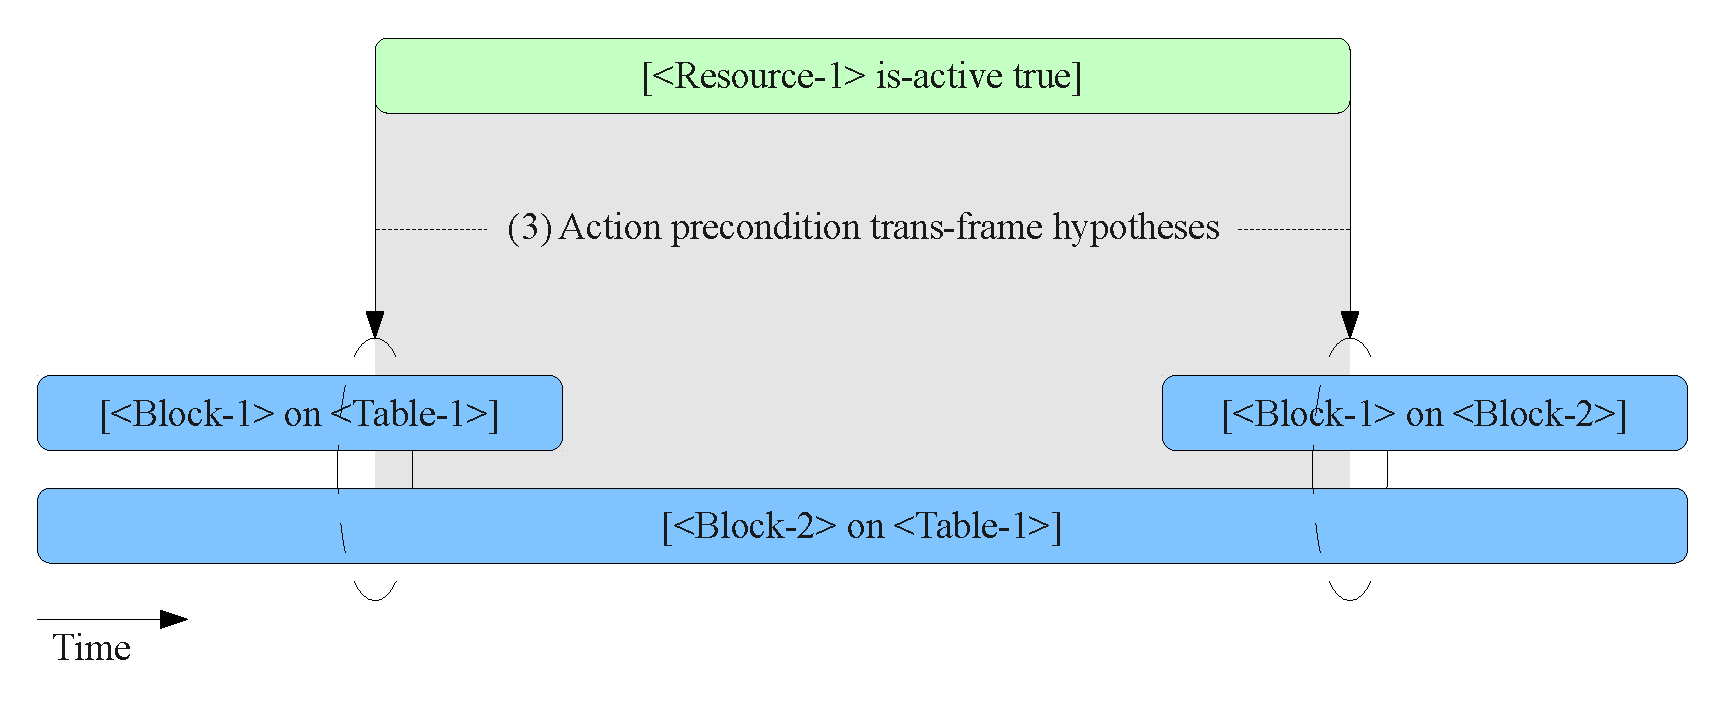
\includegraphics[width=11cm]{gfx/learning_to_plan-3-action_precondition_transframe_hypotheses}
  \caption[Action precondition trans-frame hypotheses]{Action precondition trans-frame hypotheses.}
  \label{fig:action_precondition_transframe_hypotheses}
\end{figure}

See Figure~\ref{fig:action_precondition_transframe_hypotheses}.

\begin{figure}[bth]
  \center
  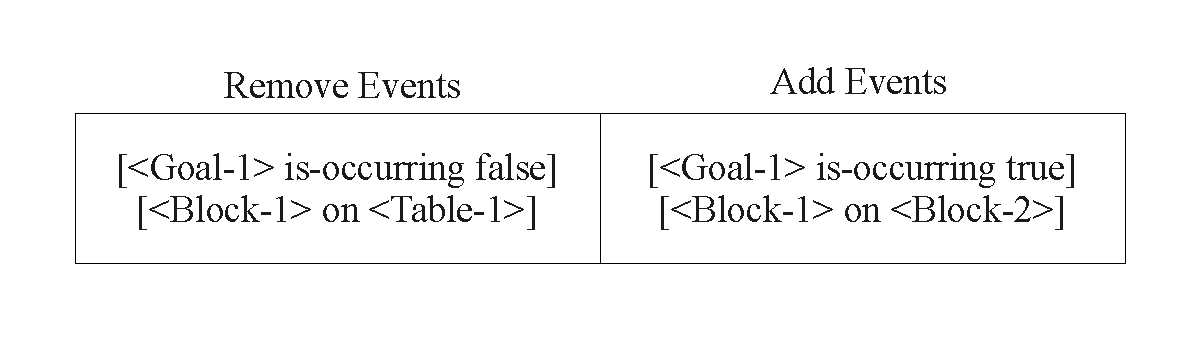
\includegraphics[width=10cm]{gfx/transframe}
  \caption[A trans-frame for an event]{A trans-frame for an event is a
    list of differences in knowledge between the beginning and ending
    of the event.}
  \label{fig:transframe}
\end{figure}

See Figure~\ref{fig:transframe}.



\subsection{Physical Goal Occurrence Hypotheses}

\begin{figure}[bth]
  \center
  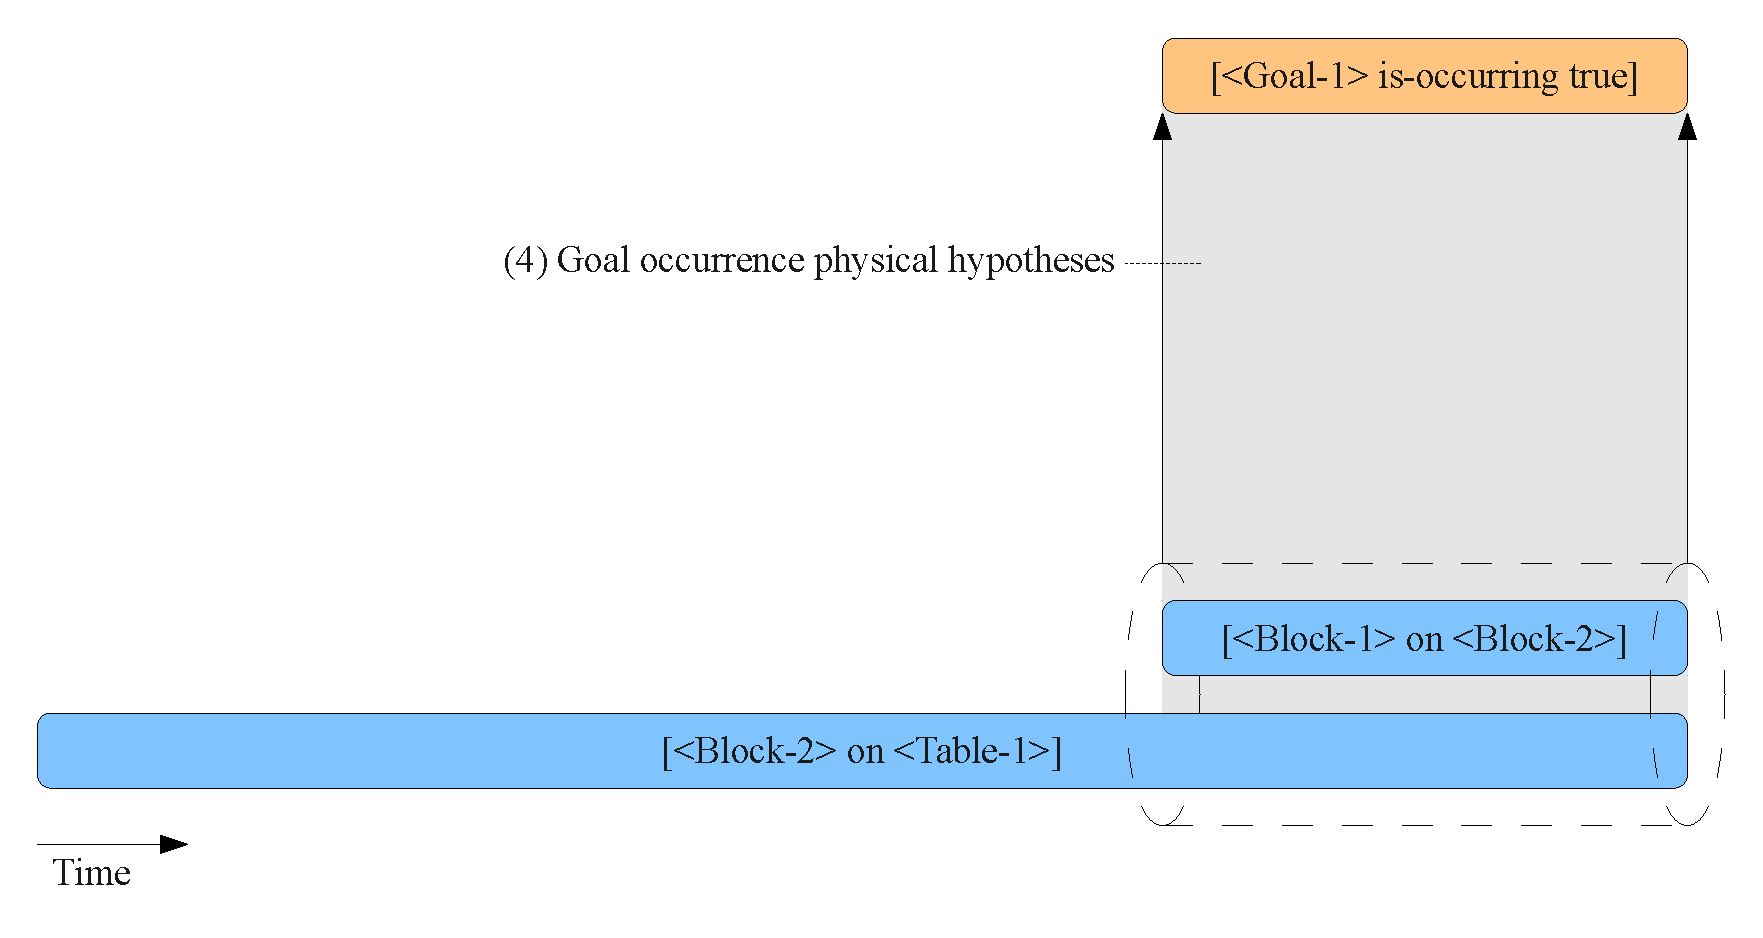
\includegraphics[width=11cm]{gfx/learning_to_plan-4-goal_occurrence_physical_hypotheses}
  \caption[Goal occurrence physical hypotheses]{Goal occurrence physical hypotheses.}
  \label{fig:goal_occurrence_physical_hypotheses}
\end{figure}

See Figure~\ref{fig:goal_occurrence_physical_hypotheses}.



\section{The Planning Process}

I have now introduced my definition of reflective event representations, 

\subsection{Partially-Ordered Plan Representation}

\begin{figure}[bth]
  \center
  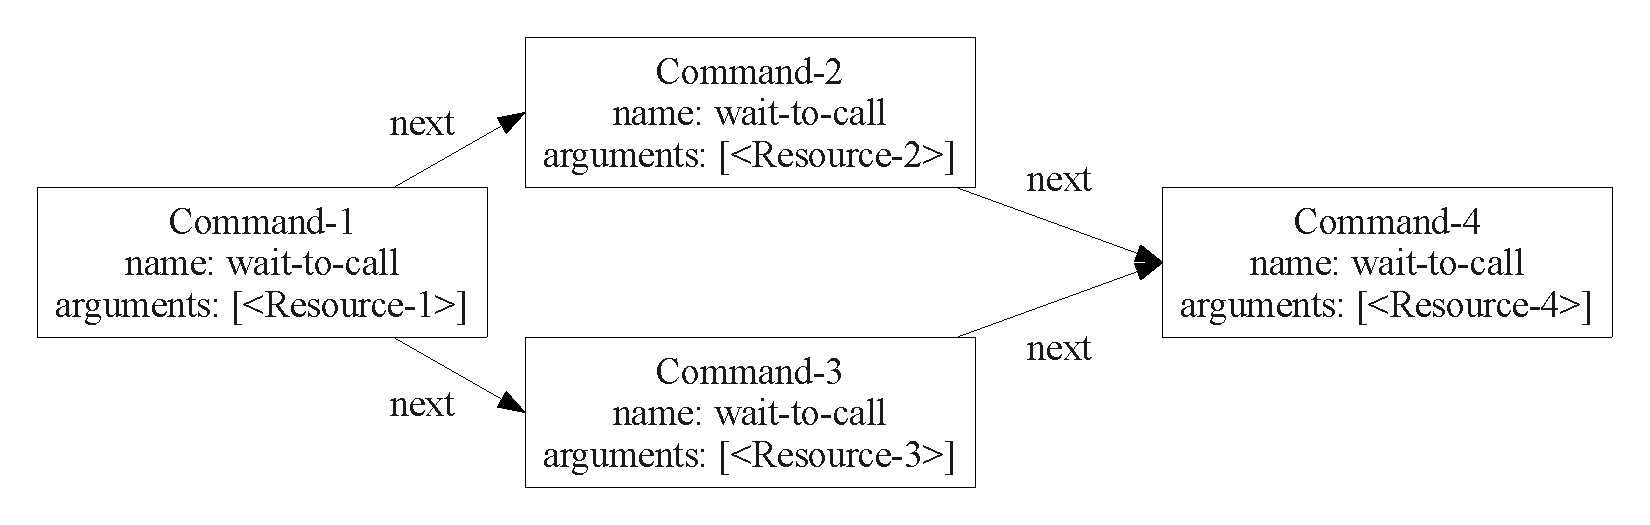
\includegraphics[width=11cm]{gfx/serial_and_parallel_plan}
  \caption[A partially-ordered plan with serial and parallel
    components]{A partially-ordered plan representation containing
    serial and parallel components.}
  \label{fig:serial_and_parallel_plan}
\end{figure}

The partially-ordered plan representation allows a partially-ordered
temporal organization for a set of commands.  A plan with a
branch-and-join control structure is shown in
Figure~\ref{fig:serial_and_parallel_plan}.


\subsection{Inferring the Effects of a Plan}
\label{sec:inferring_the_effects_of_a_plan}

\begin{figure}[bth]
  \center
  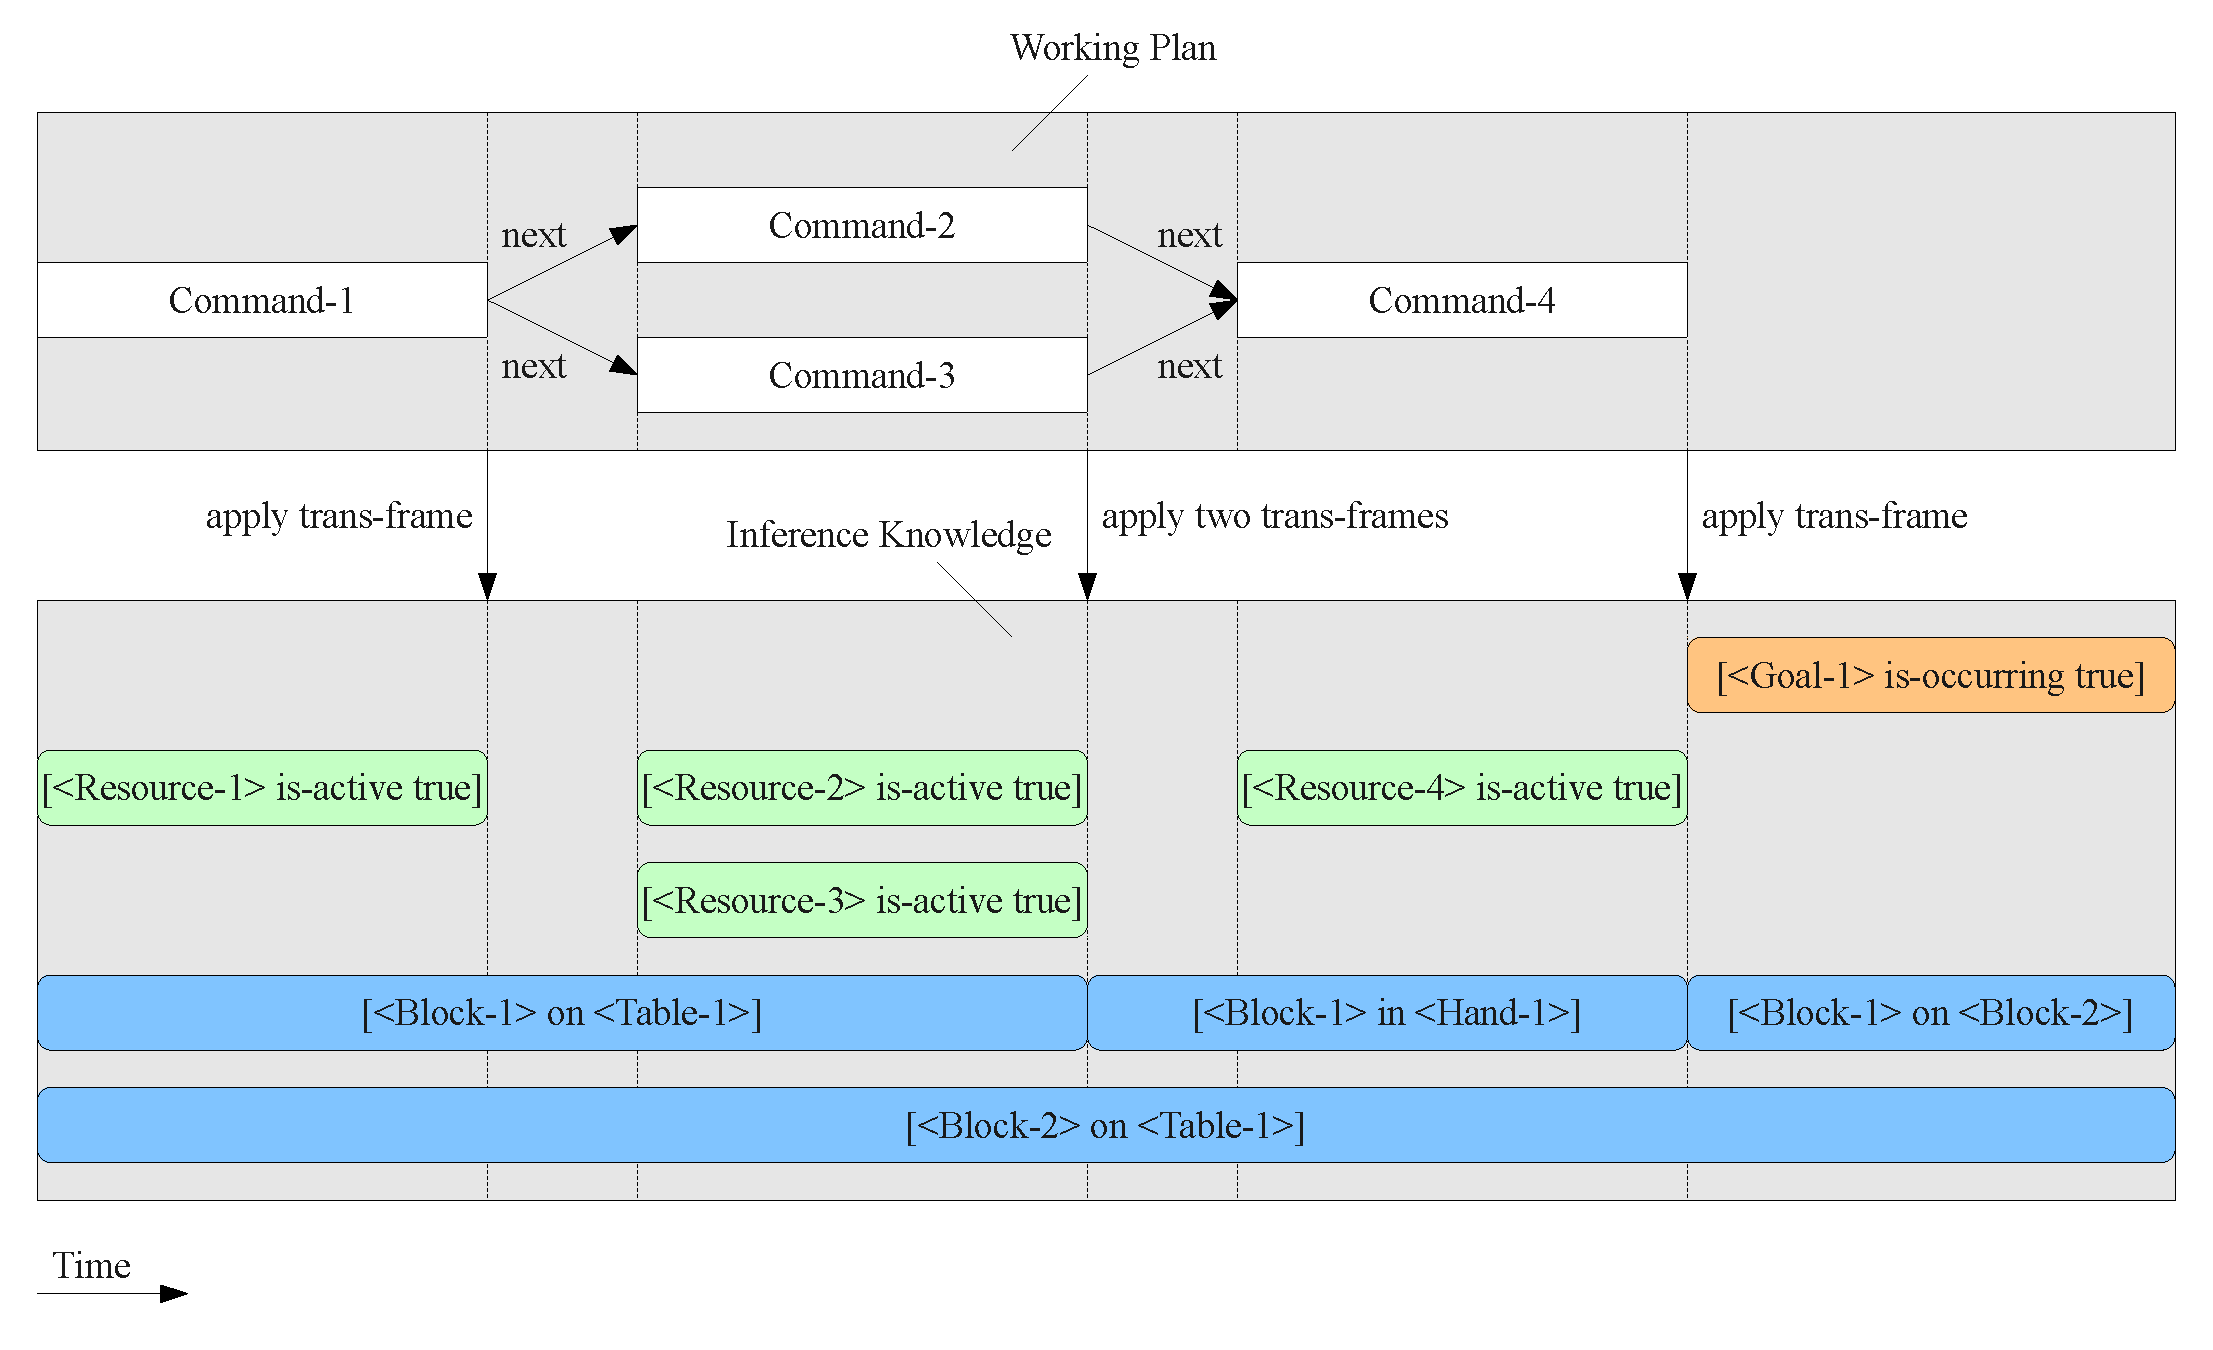
\includegraphics[width=11cm]{gfx/infer_plan_effects}
  \caption[Inferring the effects of a plan]{Inferring the effects of
    a plan.}
  \label{fig:infer_plan_effects}
\end{figure}

The planning process requires an inference algorithm to infer future
and past states based on cause-effect relationships between reflective
knowledge and physical knowledge.  Figure~\ref{fig:infer_plan_effects}
shows a possible inference for a given plan.  There are many ways to
plan and the specific planning system that I have implemented for my
experiments is discussed further in
Section~\ref{sec:details_of_inferring_the_effects_of_a_plan}.


\subsection{Planning Machine Operations}

\begin{figure}[bth]
  \center
  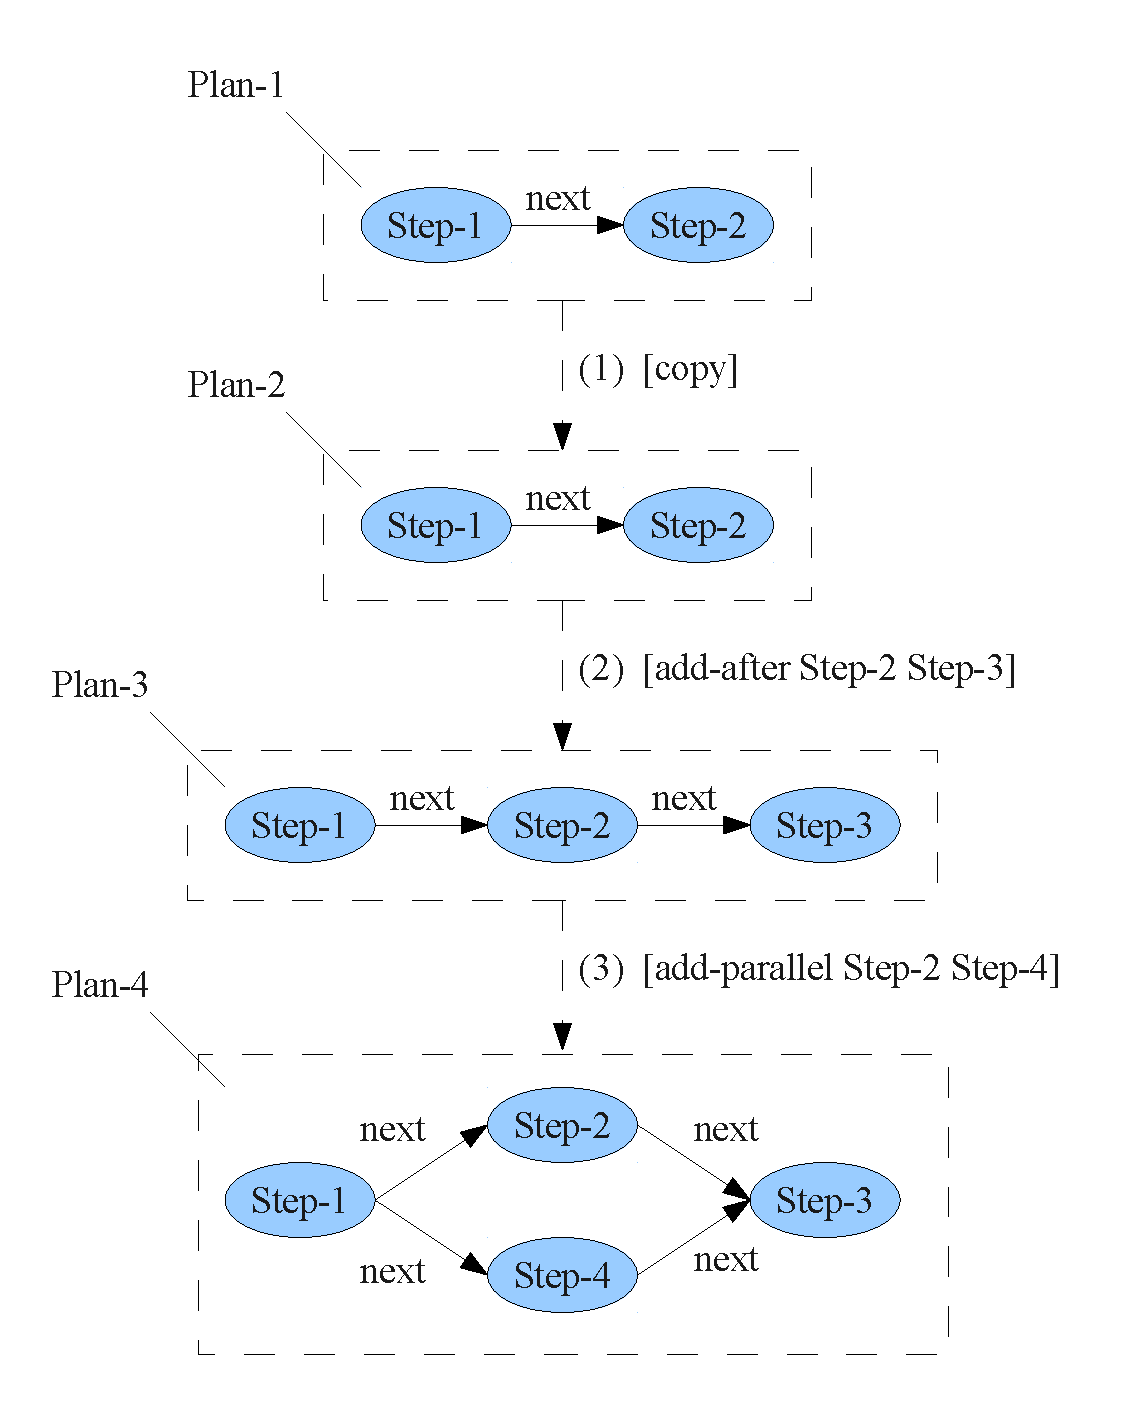
\includegraphics[height=8cm]{gfx/planning_machine_operations}
  \caption[A few planning machine operations]{A few planning machine operations.}
  \label{fig:planning_machine_operations}
\end{figure}

A few operations for manupulating partially-ordered plans are shown in
Figure~\ref{fig:planning_machine_operations}.


\section{Layering Reflective Learning}

I have now introduced how reflective representations can be used for
learning how to plan.  In this section, I will show how using the same
reflective approach to learning to plan toward goals can be used to
build another layer of reflective control on top of our planner.  This
next layer of reflective control learns to accomplish reflective goals
for the plan domain of the first-level planner.

\subsection{Planning Machine Reflective Knowledge}

The same reflective learning to plan cycle can be applied to the
actions of the planning process itself, introducing an idea of
reflective goals.  The basic four steps of the reflective learning to
plan cycle are very similar when applied to the deliberate planning
process:

\begin{enumerate}
\item{Changing reflective goal knowledge initiates causal learning.}
\item{Deliberative precondition concept for reflective goal achievement is refined.}
\item{Deliberative transition concepts for simulating deliberative action resource are refined.}
\item{Deliberative concept for reflective goal achievement is refined.}
\end{enumerate}

\begin{figure}[bth]
  \center
  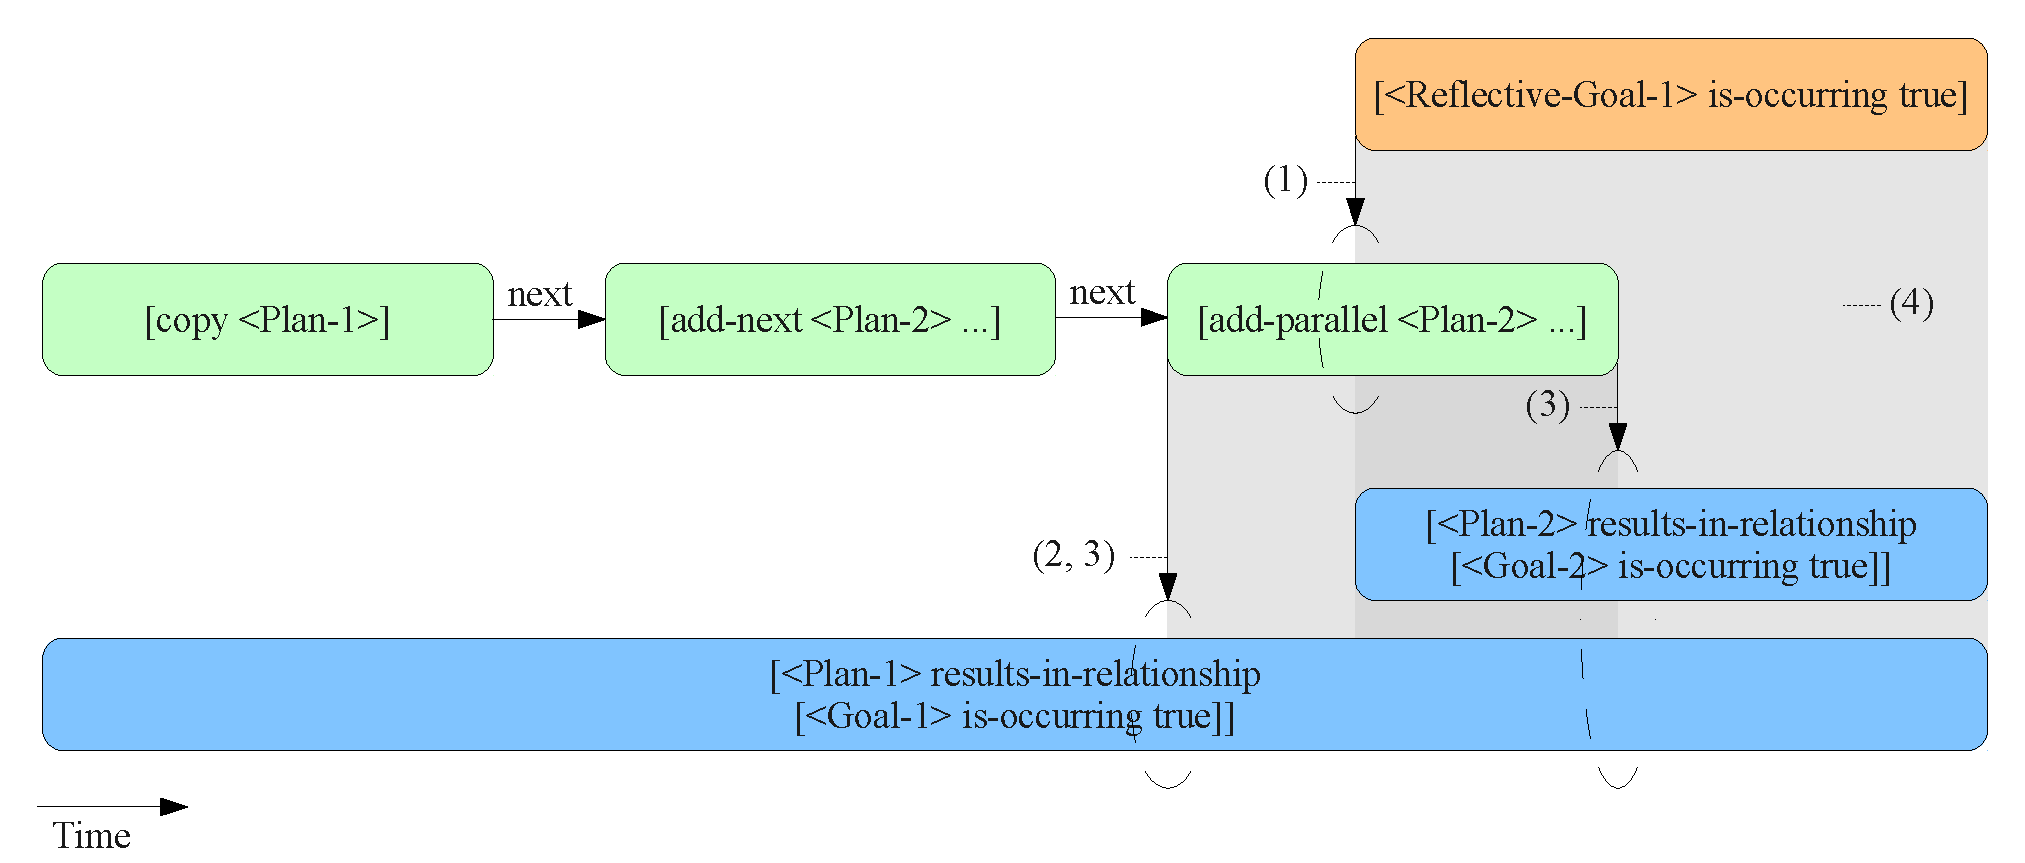
\includegraphics[width=11cm]{gfx/planning_machine_reflective_knowledge}
  \caption[Planning machine reflective knowledge]{Planning machine reflective knowledge.}
  \label{fig:planning_machine_reflective_knowledge}
\end{figure}

See Figure~\ref{fig:planning_machine_reflective_knowledge}.



